\documentclass[emulatestandardclasses]{scrartcl}
\usepackage{graphicx}
\usepackage{color}
\usepackage[ngerman]{babel}
\usepackage{hyperref}
\usepackage{fullpage}
\usepackage{calc} 
\usepackage{enumitem}
\usepackage{titlesec}
\newcommand{\todo}[1]{\textcolor{red}{TODO: #1}\PackageWarning{TODO:}{#1!}}
\date{\vspace{-3ex}}
\begin{document}

\title{
	\includegraphics*[width=0.75\textwidth]{ErstesSem/images/hu_logo.png}\\
	\vspace{24pt}
	Hegels Ph"anomenologie des Geistes - ausgew"ahlte Kapitel}
\subtitle{Proseminar SS 17\\
          Dr. Dimitris Karydas\\
          Theologische Fakult"at \\ 
          Humboldt Universit"at zu Berlin}
\author{Lennard Wolf\\
        \small{\href{mailto:lennard.wolf@student.hu-berlin.de}{lennard.wolf@student.hu-berlin.de}}}
\maketitle
\begin{abstract}

Es werden Vorrede, Einleitung und ausgewählte Abschnitte des Werkes gelesen, die mit dessen Anliegen, systematischen Aufbau und der Durchführung einiger entscheidender argumentativer Züge vertraut machen sollten. Vorgesehen sind: die sinnliche Gewissheit, Bewusstsein und Selbstbewusstsein (Herrschaft und Knechtschaft), die absolute Freiheit und das absolute Wissen. Im close reading Verfahren sollte die systematisch geleitete Bewegung, in der der Unterschied des Bewusstseins überwunden wird, an ihren Knotenpunkten nachvollzogen werden.
\end{abstract}
\newpage

\tableofcontents
\listoffigures
\newpage


\section{Einf"uhrung\\(25.04.17)}

\subsection{Organisatorisches}

\begin{itemize}
  \item Moodle-PW: bewusst (ab 27.04.)
  \item Abgabe: Essay/Protokelle zu insgesamt 10 Seiten
  \item F"ur schein der Teilnahme ist ein Protokoll abzugeben
\end{itemize}

\subsection{Einf"uhrung}

\begin{itemize}
  \item Relevanz? Wird meist fetischistisch behandelt (sowohl positiv und negativ)
  \item Teil des kulturellen/gesellschaftlichen Ged"achtnisses
  \item Ohne Systematik macht Hegel keinen Sinn (Interpretation wird schwer/unm"oglich)
  \item Ziele der Veranstaltung: Fetischmismus soll abgebaut werden (mit Duktus/Systematik vertraut machen), Verst"andnis von Hegels Pr"agung/Relevanz f"ur unsere Zeit, Kontextualisierung des Werks innerhalb der Philosophie-Geschichte (Bez"uge herstellen zum Denken seiner Zeit, und heutigem Denken/Philosophieren)
  \item Einleitung ganz am Anfang geschrieben, Vorrede ganz am Ende
  \item 1806 begonnen, Fr"uhjahr 1807 erschienen, 7 Kapitel (gro"se Kapitel am Anfang, werden immer k"urzer wegen Zeitdruck (Fortbestehen der Uni Jena war unsicher wegen der nahenden Napoleonischen Truppen))
  \item Selbstbewusstsein als Leitfaden zur gesamten Struktur der P.d.G.
  \item S. d. B.s "`Das Zweite Geschlecht"' nach selber Struktur
  \item Bestandsaufnahme "uber die Erfahrung des Bewusstseins ("`Wissenschaft "uber die Erfahrung des Bewusstseins"')
  \item Hegel in einer lebenslangen Entwicklung - \emph{kein} fertiges System $\rightarrow$ kein gro"ses einheitliches System (!)
  \item Erstes gro"ses Buch Hegels (er hat nur wenige geschrieben)
  \item Arbeit am "`System"' ab 1802/03 in zweitem Drittel der Jenaer Zeit (3 Jenaer Systementw"urfe) $\rightarrow$ dadurch bekam er eine Vorstellung davon, was ein philosophisches System ist
  \item Zeit Hegels "`Zeit der gro"sen Systeme"', Beispiel: Festschrift der deutschen Philosophie
  \item Was ist ein System? \emph{Nicht}: Menge an Prinzipien, keine Gliederung von au"sen | \emph{Sondern}: Der Innere Zusammenhang des Ganzen, "`Das Wahre ist das Ganze"', Innere Orientierung am Ganzen, was die Welt am Innersten zusammenh"alt, "`einzige Darstellungsform des \emph{Wahren}"', Wahres nicht als Gegenteil vom Falschen, sondern das Wahre arbeitet aus dem Falschen heraus
  \item Adorno: "`Das Ganze ist das Unwahre"'
  \item Kants Philosophie ist die "`Folie"' auf der Hegel sich abarbeitet, Hauptbezugspunkt ($\rightarrow$ Buch selber zeigt sein kulturelles Ged"achtnis)
  \item Das \emph{Absolute} (Wissen) als Ergebnis des Buchs, "`Kristallnetz der Verkn"upfungen"' (Marx), "`Das Wesen des Denkens"' (\emph{nicht} wo alles gleich ist)
  \item "`Ph"anomenologie des Geistes"' als Einleitung zum System
  \item Philosophie der \emph{Idee}, dessen Tr"ager der Geist ist
  \item "`Realit"at"' ist das was ist, "`Wirklich"' sind die Strukturen dahinter
  \item "`Geist"': Kulturelle Produktion der Menschheitsgeschichte, die Selbstvorstellung des Menschen "uber sich
  \item Wissenschaft ist der Geist, der sich als Weist wei"s - Kulturelle Artefakte sind Versuche der Selbstvorstellung
  \item Junghegelianer, Linkshegelianer verstanden das Buch als Geschichtsphilosophie, Dozent: "uberzeugt von dem Argumenten \emph{dagegen}: 
  \item Buch war laut hegel erst zu dieser Zeit m"oglich (nicht 20 Jahre fr"uher), denn: Protestantismus und franz. Revolution sind Voraussetzung gewesen denn: Freiheit rechtlich kodifizeirt f"ur \emph{alle} $\rightarrow$ Geist thematisiert sich selbst, ohne "au"sere Einfl"usse, totale Selbstbez"uglichkeit
  \item Was nimmt sich das Buch vor? "`Unterschied des Bewusstseins"' "uberwinden (Unterschied zwischen Bildern, die sich das Bewusstsein von der Welt macht, und dem Gegenstand selbst)
  \item Erfahrungsgeschichte--?
\end{itemize}

Das absolute? in unserer Welt?


\subsection{Einleitung}

\begin{itemize}
  \item Alle Vorraussetzungen immer hinterfragen, "`Wo kommen die her?"'
  \item 
\end{itemize}


\newpage
\section{"Uber den Professor}
Prof. Mustermann ist..


%\begin{figure}[h]
%	\centering
%	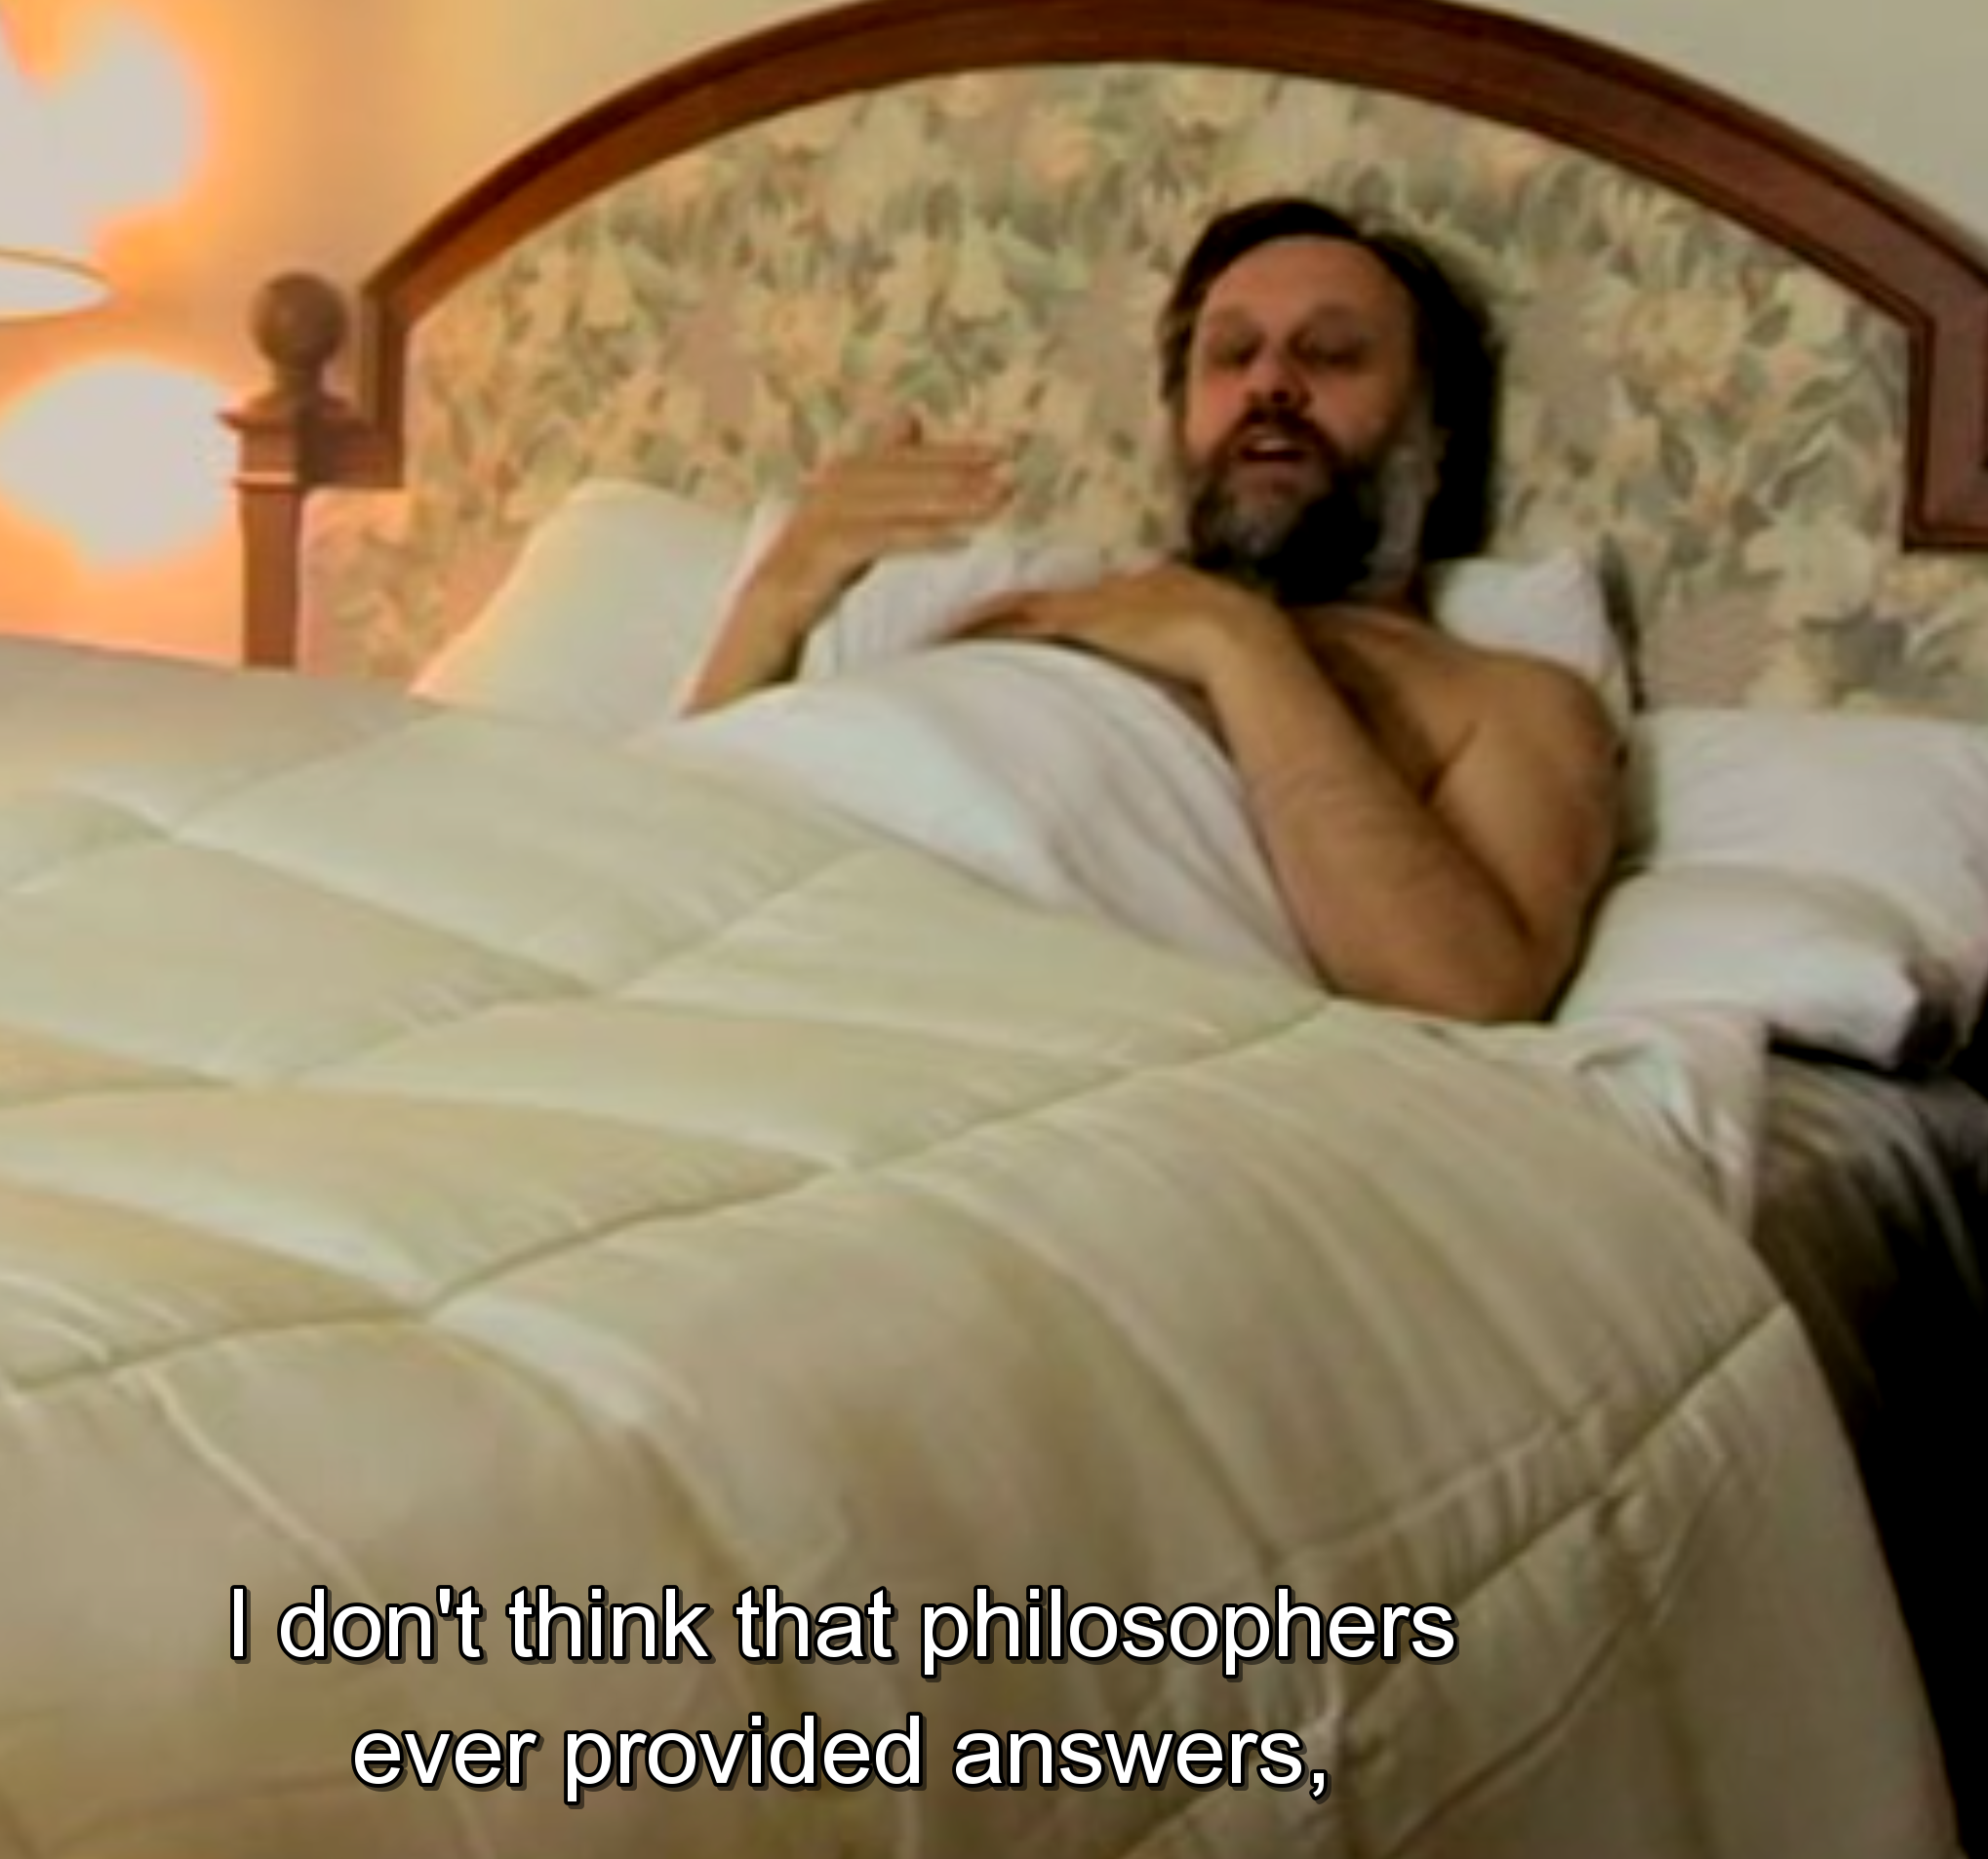
\includegraphics[width=0.5\textwidth]{images/template.png}
%	\caption{Template Bild}
%	\label{fig:template}
%\end{figure}

\end{document}
